
\documentclass[phd,tocprelim]{cornell}

\let\ifpdf\relax
\usepackage{url}
\usepackage{graphicx}
\usepackage{color}
\usepackage{float}

\usepackage[section]{placeins}
\usepackage{graphicx,pstricks}
\usepackage{graphics}

\usepackage{moreverb}
\usepackage{subfigure}
\usepackage{epsfig}
\usepackage{txfonts}
\usepackage{multirow}
\usepackage{todonotes}
\usepackage{glossaries}
\usepackage[none]{hyphenat}
\usepackage{setspace}
\usepackage{hyperref}
\usepackage{listings}



\graphicspath{ {Images/} }

\usepackage[utf8]{inputenc}

\tolerance=9999


\bibliographystyle{plain}
%\bibliographystyle{IEEEbib}

\usepackage{listings}
\usepackage{color}

\makeglossaries




\definecolor{dkgreen}{rgb}{0,0.6,0}
\definecolor{gray}{rgb}{0.5,0.5,0.5}
\definecolor{mauve}{rgb}{0.58,0,0.82}
\renewcommand{\topfraction}{0.85}
\renewcommand{\textfraction}{0.1}
\renewcommand{\floatpagefraction}{0.75}
\renewcommand{\chaptername}{Kapittel}

\title{Forbedret brukervennlighet innen alternativ og supplerende kommunikasjon for mennesker med forsinket 
eller avvikende språk- og kommunikasjonsutvikling.} 

\author{Morten Holst Øvrebø}

\begin{document}

\begin{figure}[ht!]
\centering

\includegraphics[width=80mm]{HIB_sort_hovedlogo_engelsk}
\end{figure}


\maketitle


\begin{abstract}
Abstract here
\end{abstract}
\begin{acknowledgements}
acknowledgements here. 
\end{acknowledgements}

\newglossaryentry{isaac}{name=ISAAC, description={ International Society for Augmentative and Alternative Communication}}

 \newglossaryentry{aske}{name=ASK, description={alternativ og supplerende kommunikasjon}}
 
 
  \newglossaryentry{PCCR}{name=PCCR, description={Pupil Centre Cornea Reflection, er en teknikk som brukes til ikke-forstyrrende øyesporing}}


  \newglossaryentry{WPF}{name=WPF, description={Windows  Presentation  Foundation}}

  \newglossaryentry{XAML}{name=XAML, description={Extensible Application Markup Language}}
 
\printglossaries
\contentspage
\figurelistpage
\listoftodos

\normalspacing \setcounter{page}{1} \pagenumbering{arabic}
\pagestyle{cornell} \addtolength{\parskip}{0.5\baselineskip}



\chapter{Introduksjon}




\section{Motivasjon}
\label{sec:motivasjon}

Tale og språk tillater oss å rekke ut til andre og leve tilfredstillende liv som uavhengige medlemmer av samfunnet. Språk gir oss identitet, felleskap  og tilhørighet. Det er derimot flere som blir hindret i å uttrykke seg gjennom tradisjonelle kommunikasjonsformer på grunn av ulike funksjonshemninger  \cite{tobii}. De har derfor et behov for alternativer for å kunne kommunisere. Folk med syn eller hørselsskader har tatt i bruk gester, tegnstøtte eller tegnspåk. Andre har måttet bruke mer håndgripelige hjelpemidler. Ett kjennetegn ved disse formene for kommunikasjon er at de krever at brukeren har muskelkraft. Et krav som utelukker  personer med ALS, cerebral parese (CP), autisme og afasi eller de som har hatt hjerneslag. Folk med disse funksjonshemningene har ofte motoriske utfordringer som hindrer dem fra nettopp verbal og kroppspråklig kommunikasjon. Ved hjelp av data- og øyestyrings-teknologi er det mulig for flere av disse menneskene å kommunisere. Utfordringen er at feltet er relativt ungt og nåværende forskning har hovedsaklig blitt gjort på voksne uten funksjonshemninger (OBS! pass på at du ikke gjør det samme eller evt fjerner denne) \cite{aac}. I dette prosjektet vil fokus bli rettet mot barn som ikke har tilgang på tradisjonelle kommunikasjonsformer.




\section{Målgruppe}

I kapittel \ref{sec:motivasjon} nevnes det at det er flere unge mennesker som helt eller delvis mangler tale. Som en konsekvens av dette har de behov for andre uttrykksformer for å kommunisere. Alternative uttrykksformer kan være håndtegn, symboler eller fotografier. Slike utradisjonelle uttrykksformer går under fellesbetegnelsen alternativ og supplerende kommunikasjon (\gls{aske}).
Personer bruker ASK enten fordi det er et behov for å erstatte talen eller for å supplere utydelig eller svak tale.

International Society for Augmentative and Alternative Communication (\gls{isaac}) \cite{HvaErASK} definerer ASK som alt som hjelper en person til å kommunisere effektivt når tradisjonelle måter å kommunisere på ikke strekker til.

Målgruppen i denne avhandlingen er personer som har behov for ASK systemer. Mer spesifikk vil rapporten være rettet mot: (A) Mennesker som ikke har mulighet for tale- og kroppspråk,  (B) personer ikke håndterer skriftspråk og (C) at de er nybegynnere på symbolbasert kommunikasjon. Dette gjelder hovedsaklig barn i alderen 2 til 5 år, men også eldre med mentale begrensninger. Videre i dette prosjektet vil personer som møter disse kriteriene bli omtalt som barn med komplekse kommunikasjonsbehov. 

\section{Mål}
\label{sec:goal}

Målet med dette prosjektet er å lage et ASK-system som hjelper barn med komplekse kommunikasjonsbehov å kommunisere. Systemet som skal utvikles tar utgangspunkt i et eksisterende program som heter Sono Flex (se figur ~\ref{fig:SonoFlex}). Programmets hovedfunksjon er å konvertere tekst og symboler til tale, samt at det innholder et rikholdig utvalg av funksjoner for læring, omgivelsekontroll og elektronisk fjernkommunikasjon \cite{TobiiCommunicator}. Formålet med systemet er å hjelpe brukeren å kommunisere med symboler. Der et symbol representerer et ord eller et konsept som "hjem" eller "min mor". Problemstillingen er at når brukerens aktive vokabular vokser, så vil også antallet symboler øke. Dette gjør at det oppstår et behov for å dele symbolene inn i kategorier og flere visninger.

Light og Drager \cite{aac} argumenterer at videre forskning innen ASK teknologi må fokusere på forbedret design, for bedre å kunne møte behovet fra unge barn og eldre nybegynnere. I dette prosjektet er målet å designe og prototype mulige løsninger som reduserer den mentale belastningen på brukeren, mens han bruker et stort vokabular, med eller uten en øyestyrings enhet.

\begin{figure}[ht!]
\centering
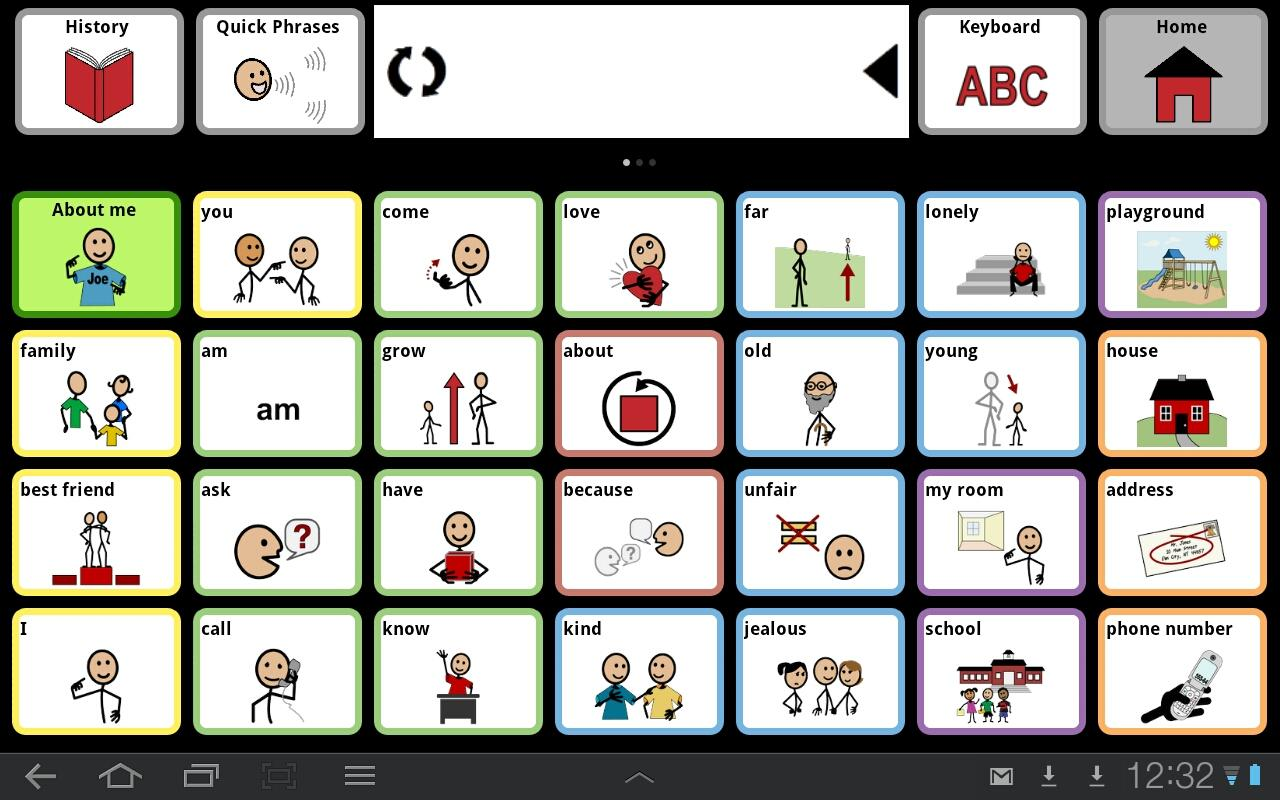
\includegraphics[width=150mm]{SonoFlex2}
\caption{Skjermdump av ASK programvaren Sono Flex}
\label{fig:SonoFlex}
\end{figure}


\section{Forskningspørsmål}
\label{sec:ResearchQuestion}

For å forske på mulige løsninger som forbedrer ASK-systemer vil en rekke funksjoner integreres i prototypen. Funksjoner som vil bli utprøvd og forsket på er følgende:


\begin{enumerate} 
\label{lst:features}
\item Forbedret visualisering. Undersøk mulige fordeler forskjellige visualisering effekter kan ha på navigering innen og mellom sider og kategorier.
\item Lydeffekter. Undersøk mulige fordeler forskjellige lydeffekter kan ha på navigering innen og mellom sider og kategorier.
\item Optimal organisering og kategorisering. Hvordan skal knapper bli organisert og kategorisert for best å legge til rette for og forenkle navigasjon
\item Brukertilpasning. Mennesker har forskjellige preferanser. Undersøk mulighetene for tilpasning av symbolstørrelse, animasjonsfart, farger o.s.v. 
\end{enumerate} 


Forskningen vil bli gjort ved å implementere et program basert på en eksisterende løsning. De ulike forbedringene beskrevet i (1),(2) og (3) vil bli integrert. Samtidig vil det også være mulighet tilpasse etter ønske (4). 


\section{Forskningsmetode}

Som nevnt i seksjon \ref{sec:ResearchQuestion}, er oppgaven å forbedre en type kommunikasjons programvare for mennesker med komplekse kommunikasjonsvansker. For å undersøke innvirkningene til de forskjellige funksjonene, vil de prøves ut på en testgruppe.
For å få til dette, vil et utvalg av deltakerene prøve systemet uten tilleggsfunksjonene, mens de gjenværende vil forsøke med funksjonene. Mens deltagerne kjører programmet vil deres interaksjon med bli automatisk lagret i logg. Informasjonen fra undersøkelsen vil vise hvordan brukeren navigerte og hvor lang tid de brukte. Dette kan igjen brukes til å verifisere om en funksjon er en forbedring eller ikke.


\chapter{Bakgrunn}

I dette kapittelet vil de viktigste konseptene, fenomenene og teknologiene bli beskrevet og eksisterende  forskning som er relevant for oppgaven. 

\section{Kommunikasjonsform: Symboler}

De som ikke har mulighet til å bruke skrift som kommunikasjonsform kan bruke tegnsystemer. Det eksisterer tre typer tegnsystemer: håndtegn(manuelle tegn) som innebærer å bruke håndbevegelser, materielle tegn vil si at en bruker fysiske objekter som brikker eller figurer og den siste er; grafiske tegn som innebærer at en bruker symboler. I denne rapporten er vil symboler bli brukt som kommunikasjonsform. Her representerer symboler et ord, frase, uttrykk eller setning. Ifølge ISAAC \cite{Tegnsystemer} er grafiske tegn brukt av mennesker med store bevegelsesvansker som gjør at de har utfordringer med å lage manuelle tegn, og mennesker med forståelsesvansker som følge av lærehemning.

De vanligste grafiske tegnsystemene på markedet er fotografi, pictogram, Picture Communication Symbols(PCS), Widgit, SymbolStix og Bliss \cite{GrafiskTegn}. I prosjektet brukes SymbolStix (se figur \ref{fig:katt}). Grunnen til dette er at Sono Flex bruker dette tegnsystemet.


\begin{figure}[ht!]
\centering
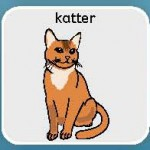
\includegraphics[width=50mm]{katt}
\caption{Et eksempel på et symbol som blir brukt i det grafisk tegnsystemet SymbolStix}
\label{fig:katt}
\end{figure}

\section{Interaksjonsform: Øyestyring}

Menneske-maskin-interaksjon fungerer ved at en person gir maskinen en kommando, og maskinen svarer med en respons. For at et menneske skal kunne gi en maskin ordre, er det nødvendig at maskinen har en inputenhet som tolker beskjedene fra brukeren, slik at at datamaskinen forstår dem.  Som regel er dette tradisjonelle enheter som tastatur og mus. Det eksisterer derimot mangfoldige måter å samhandle med en maskin på. I denne rapporten vil brukerinput bli gitt ved en øyestyringsenhet.  Ved å fange opp brukerens skuepunkt av et videokamera og infrarøde lys, er det mulig for maskinen å beregne hvor på monitoren personen ser. Dette gjør interaksjon mellom dem mulig. En knapp vil for eksempel bli aktivisert ved at brukeren ser på den en hvis periode. 




\section{Forskning}


\subsection{Organisering}


I 1926 kartla Smith\cite{Smith} barns vokabularutvikling fra alderen 1 til 5 år . Resultatene (se tabell \ref{fig:BarnVak}) viste at allerede i en alder av 3 er det vanlig å ha en gjennomsnittlig forståelse for cirka 900 ord. Forskningen er 88 år gammel, men viser omfanget av utfordringen barn har i møte med symbolbasert kommunikasjon. Mens et barn med taleevne kun trenger å finne ordet i hukommelsen, må barn som bruker symboler først finne det og deretter lokalisere det representative symbolet. 

I applikasjonen som skal utvikles vil symbolene bli presentert i en tabell. Antall symboler som får plass i tabellen begrenses av skjermens fysiske størrelse og at de må være store nok til at brukeren har mulighet til å se  og samhandle med dem. En slik tabell med symboler vil herfra bli referert til som en side. For hver setning brukeren vil uttrykke må han navigere seg igjennom flere av disse sidene for å finne symbolene som representerer ordene i setningen. Det er derfor essensielt at organiseringen legger til rette for akkurat dette, og ikke vanskeliggjør barnets evne til å lokalisere, velge og bruke symbolene.

\begin{table}[h]
\begin{tabular}{llllllllll}
\hline
Alder (År, Måneder) & 1 & 1,6 & 1,9 & 2,0 & 2,6 & 3,0 & 3,6  & 4,0  & 5,0  \\ 
Antall ord          & 3 & 22  & 118 & 272 & 446 & 896 & 1222 & 1540 & 2072 \\ 
Økning              & 2 & 19  & 96  & 154 & 174 & 450 & 326  & 330  & 532  \\ \hline
\end{tabular}
\caption{Tabell som viser vokabular vekst hos barn.  Smith \cite{Smith} sitert av Dale \cite{Dale} }
\label{fig:BarnVak}
\end{table}



Drager og Light \cite{aac} viser til at det inntil nylig var gjort lite forskning på layouts og organisering for barn eller om faktorene som spiller inn når det gjelder lokalisering og bruk av målobjektene. Målobjektet er symbolet som brukeren ønsker å uttrykke. Wilkinson og Jageroo \cite{Wilkinson2006} har undersøkt hvilke påvirkning farge har som en faktor når det kommer til organisering og hvordan elementer skal fordeles. De kom frem til at fargehint spiller en viktig rolle innen visuell prosessering  og hukommelse. Ved å legge til en farge ved elementene i tabellen over symboler, påvirket det nøyaktigheten og effektiviteten til barn i 4-5 års alderene i å finne målobjekt. Eksempelvis kan man gi symboler som representerer verb en grønn farge, adjektiv en blå, pronomen gul o.s.v. Fenomenet kalles Fitzergald Key og gjør at barn mer presist og raskere lokalisere målobjektet. Scally \cite{Scally} argumenterer for at farge ikke nødvendigvis er den eneste variabelen som må vurderes. Andre skjerm variabler som kan påvirke læring og bruk er: bakgrunn, kanter/grenser, form, tekstur, størrelse, posisjon, bevegelse og animasjon. Videre undersøkelser må til for å avgrense effektene av disse funksjonene for å kunne optimere designet til ask-systemer.


\subsection{Navigasjon}
\label{subsec:navigasjon}

Hvis en tar med alle typene frukt så vil det ikke være plass til alle symbolene på en side, dette gjør at de må deles opp over flere sider.Konsekvensen er at brukeren må ha mulighet til å navigere mellom disse sidene for å finne ønsket symbol. Siden antallet symboler det er plass til på hver side begrenses av skjermstørrelsen og brukerens syn, er spørsmålet hvor mange symboler bør plasseres på hver side med tanke på effektivitet. Drager og light med kollegaer undersøkte nettopp dette. Resultatene indikerte at barn i alderen 2-5 hadde større vanskeligheter for å lokalisere korrekt side fra en meny med 4 symboler enn en så lokalisere målobjektet når på korrekt side ut av et valg på 12 til 30 symboler, til tross for at sannsynligheten for å finne korrekt side er 25 prosent er mye større enn å finne korrekt symbol 0.03 - 0.08 når en først er på rett side.

For barn kan det å navigere være ekstra vanskelig. Dette kommer av flere grunner: (a) de må ha en konseptuell modell av de gjemte sidene i systemet i minnet. Med andre ord forstå hvordan de mest effektivt kan komme seg fra forsiden til ønsket symbol. (b) De må forstå forholdet mellom representasjon brukt på menysiden og de gjemte sidene i vokabularet. Er det symbolet som har bilde av et kjøkken eller av en butikk som leder til symbolet eple? I denne rapporten vil disse utfordringene bli undersøkt.




\chapter{Øyesporing}

Øyesporing refereres ofte til teknikken brukt til å fange og måle øyebevegelser \cite{Calibration}. Målet med dette kapittelet er å gi en beskrivelse av hvordan øyesporing fungerer og enheten som brukes i denne avhandlingen - samt en forklaring av viktige konsepter.


\section{Hvordan fungerer øyet?}

Å forklare hvordan øyet fungerer i detalj er utenfor denne rapportens omfang. Det vil derfor kun gis en høynivå forklaring av hvordan det fungerer for å kunne forstå det som er nødvendig i henhold til rapporten. 

\subsection{Synsfelt}

I en artikkel skrevet av Tobii \cite{Calibration} sammenlignes øyet med et fotoapparat på grunn av dens mange likhetstrekk. Når lys treffer et objekt reflekteres dette, det reflekterte lyset reiser så gjennom en linse og ender opp i øyet. Linsen prosjekterer lyset den mottar på en lyssensitiv overflate. Denne overflatens oppførsel er også det som skiller øyet fra fotoapparatet. For i motsetning til et kamera er ikke overflaten like sensitiv overalt i øyet.  Dette gjør at menneske kan tilpasse synet etter hvor mye lys som er tilgjengelig. En bieffekt er at det også resulterer i at menneske kun kan se klart i begrensede områder av synsfeltet. Figur \ref{fig:visueltArea} illustrerer hvordan synsfeltet hos menneske er delt inn etter klarhet. (F) representerer det foveale området. Dette er området man fokuserer på og oppfatter klarest. Det er hovedsaklig fra dette området visuell data hentes fra . (Pf) viser det parafovela omårdet, som kjennetegnes ved at uskarpheten øker til man kommer til det perifere området. (P) Det perifere området, også kjent som sidesynet, fungerer kun bra til å fange opp bevegelser og kontraster.

\begin{figure}[ht!]
\centering
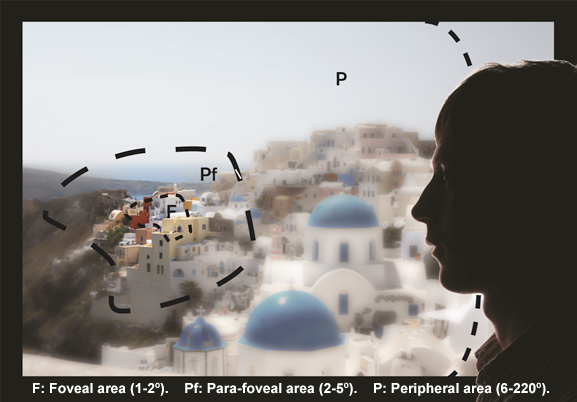
\includegraphics[width=65mm]{fovealArea}
\caption{Bilde/Illustrasjon av menneskelige synsfelt \cite{VisualImage}}
\label{fig:visueltArea}
\end{figure}

\subsection{Fikseringer og sakkader}

Det foveale området er som nevnt det området det registreres mest visuell data. Området står derimot for mindre 8 prosent av synsfeltet. Dette gjør at for å kunne innhente informasjon av interesse fra andre deler av synsfeltet må det flyttes inn i  det foveale området. For å gjøre det brukes øyeoperasjoner kalt fikseringer og sakkader. Fikseringer er pauser fra bevegelsen på et område, sakkader er hurtige bevegelser mellom fikseringene \cite{Calibration}.


\section{Hvordan fungerer øyesporing?}

Øyesporing er som tidligere nevnt teknikken brukt til å fange og måle øyebevegelser.
Det finnes derimot flere fremgangsmåter. I denne oppgaven vil det brukes en ikke-forstyrrende øyestyringsenhet. Dette gjør at brukeren i prinsippet ikke skal legge merke til enheten. For denne typen øyesporing er det mest vanlig å bruke en teknikk som heter Pupil Centre Cornea Reflection (\gls{PCCR}) \cite{Calibration}. Teknikken fungerer ved at en lyskilde belyser øyet for at refleksjonene skal bli klare og synlige. Et kamera tar deretter bilde av refleksjonene fra øyet. Bildet blir så brukt til å identifisere lysets refleksjon på hornhinnen og pupillen. Når en vet vinkelen mellom hornhinnen og pupillen er det mulig å regne ut en vektor. Vektoren sammen med andre geometriske egenskaper ved refleksjonene gjør det mulig å kalkulere ut blikkretningen(Der brukeren ser) \cite{Calibration}.


\subsection{Utfordringer}

En utfordring ved øyesporing er blunking. Blunking er et er en kortvarig sammentrekning av øyelokket, noe som gjør at øyet ikke vil gi refleksjon som kamera kan fange, og derfor ikke ha koordinater på hvor brukeren ser. Dette løses under analysen. Ved at og bruke koordinatene og øyets hurtighet før øyelokkene trakk seg sammen kan man ekstrapolere seg fram til en tilnærmet korrekt fiksering. 

\section{Tobii PCEye Go}

I denne rapporten brukes øyesporingsenheten Tobii PCEye GO, som vist i figur \ref{fig:tobiiPc}. Enheten kommer separat og kobles til datamaskinen via USB. Dette er som tidligere nevnt et ikke-forstyrrende apparat. Et eksempel på det motsatte ville vært et par briller som ble brukt til å spore øyebevegelser. 



\begin{figure}[ht!]
\centering
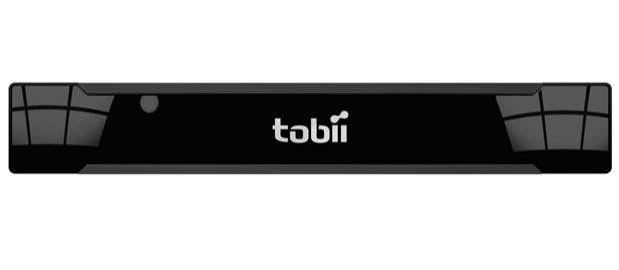
\includegraphics[width=50mm]{TobiiEyeGo}
\caption{Bilde av øyestyringsenheten Tobii PCEye Go}
\label{fig:tobiiPc}
\end{figure}


\subsection{Tobii blikkprogramvare}
\label{subsec:blikk}

Sammen med Tobii PCeye go følger det med programvare for å kontrollere applikasjoner som bruker sporingsenheten. Den består av følgende komponenter: 

\begin{itemize}
\item [Blikk interaksjonsserver] en sentral HUB som tilbyr klient applikasjoner øyesporingsdata. 
\item [Blikk interaksjons innstillinger] Et kontrollpanel for interaksjons innstillinger og oppgaver relatert til øyesporing
\item [Windows Kontroll] Tilbyr blikk interaksjon for standard Windows applikasjoner, ergo vanlige applikasjoner som ikke er laget for øyesporings interaksjon.
\end{itemize}

I denne rapporten vil kun førstnevnte være relevant. Ettersom applikasjonen er spesialisert til blikk interaksjon og ikke er en standard Windows applikasjon.

\subsection{Blikk Interaksjonsserver}

Blikk interaksjons-serveren er som nevnt i seksjon \ref{subsec:blikk} en HUB for programvaren, eller kjernen. Hovedformålet til denne komponenten er å samhandle med Øye-sporingsenheten og tilby interaksjonsfunksjonalitet for å kontrollere Windows baserte applikasjoner som vil bruke sporingsdata. I tilegg er det denne komponenten som tar seg av kalibrering, sporingsstatus - samt bruker og applikasjons innstillinger.

\subsection{Tobii Eye Control API }

Figur \ref{fig:overview} viser hvordan blikk interaksjonsserveren eksponerer funksjonalitet til en klient-applikasjon gjennom et APIet, som er kalt Tec API. For å ta i bruk TecAPIet tilbys to aksess punkter. Et gjennom .NET plattformen kalt TecClient og et for C dynamisk link library kalt MPACI.  Den praktiske betydningen, er at man kun kan bruke APIet ved å skrive i C eller .NET teknologier. I denne rapporten vil kun sistnevnte være interessant, altså .NET APIet kalt TecClient.


\begin{figure}[ht!]
\centering
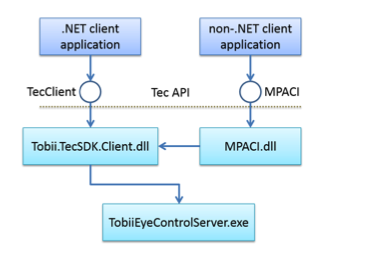
\includegraphics[width=100mm]{SoftwareArchitectureOverview}
\caption{Bilde som viser programvare arkitekturen til blikk programvaren}
\label{fig:overview}
\end{figure}


\subsection{TecClient}

TecClient støtter to GUI rammeverk; Windows Presentation Foundation (\gls{WPF}) og Windows Forms. 
 (kilde dokumentasjon).  Samhandling mellom applikasjonen og TecClienten skjer gjennom et konsept som de har valgt å kalle TecClients verktøykasse. De ulike verkøys klassene er presentert i figur \ref{fig:toolbox}. 

\begin{figure}[ht!]
\centering
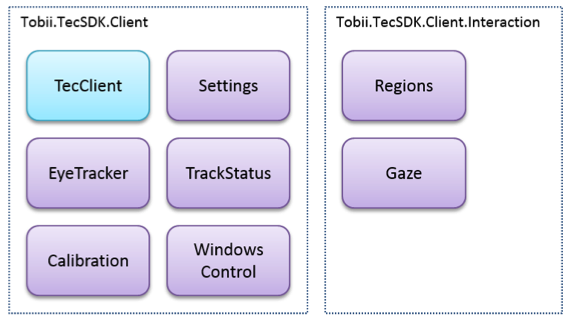
\includegraphics[width=100mm]{Toolbox}
\caption{Verktøy klassser som er tilgjengelige gjennom TecClient komponenten verktøyskasse}
\label{fig:toolbox}
\end{figure}


\subsubsection{EyeTracker}
Gir informasjon om den aktuelle øyesporingsenheten.

\subsubsection{Kalibrering}
Tilbyr tilgang til kalibrerings funksjonalitet og innstillinger som kan bli brukt for å kontroller hvordan kalibreringen er gjort.

\subsubsection{Settings}
Settings gir tilgang til bruker og klient innstillinger. Med mulighet til å hente nåværende bruker, alle bruker med funksjonalitet til å legge til og fjerne brukere og nåværende klient.

\subsubsection{Trackstatus}
Tilbyr metoder, egenskaper og hendelser for å kontrollere sporingsstatus vinduet. 


\subsubsection{Regions}
Tilbyr metoder, egenskaper og hendelser relatert til interaksjonsregioner. (1) Legge til og fjerne interaksjonsregioner, (2) hente informasjon om fokus og (3) søke etter interaksjonsregioner.

\subsubsection{Gaze}
Eksponerer blikkdata, både filtrert og ufiltrert. 


\chapter{Tobii Sono Flex}

I dette kapittelet vil den eksisterende løsningen sono flex bli diskutert. Det vil bli gitt en grundig analyse av problemstillingen og fremgangsmåte presentert.


\section{Tobii Sono Flex}
\label{chap:Tobii-Sono-Flex}


Programvaren som det tas utgangspunkt i heter Tobii Sono Flex,  og er et systematisert symbolforråd og et verktøy for alternativ og supplerende symbolspråk. Sono Flex har som mål å tilby et språk til personer som ikke enda kan lese og skrive. 

Applikasjonen fungerer som et tastatur, men istedenfor bokstaver er knappene ord med en visuell representasjon av ordet. Brukeren trykker på knappene som utgjør setningen han vil uttrykke, så vil programvaren gjøre om setningen til tydelig tale.  Systemet er spesielt utviklet for barn og unge med med sammensatte kommunikasjonsvansker, som trenger et ordforråd for å videreutvikle språk- og kommunikasjonsferdigheter. Sono flex kan ses på som en nybegynnerpakke med en lav læringskurve som skal gjøre brukeren klar for mer avanserte systemer. 


\subsection{Brukergrensesnitt}

Brukergrensesnittet til Sono Slex består av to hovedkomponenter: en menylinje og en symboltabell. 


\subsubsection{Menylinje}

Figur \ref{fig:menylinje} viser menylinjen.  Denne består av 5 elementer.  Kun de midterste er av interesse, disse  er statiske og følger applikasjonen hele tiden. Det hvite feltet i midten viser symbolene som brukerene har trykket på, og vil herved bli referert til som setningslisten. Symbolene som vises vil komme ut i form av tydelig tale ved å trykke på selve feltet. Knappen på venstre side av setningslisten (clear all), vil ved interaksjon tømme setningslisten. Mens knappen på høyre side vil kun fjerne det siste symbolet brukeren trykket på.


\begin{figure}[ht!]
\centering
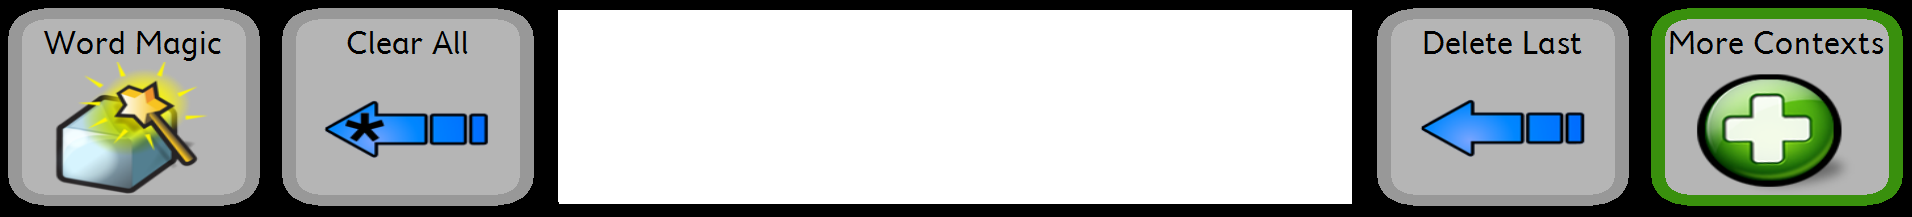
\includegraphics[width=100mm]{menylinje}
\caption{Skjermdump av menylinjen til programvaren Sono Flex}
\label{fig:menylinje}
\end{figure}




\subsubsection{symboltabell}
\label{subsubsec:symboltabell}

Figur \ref{fig:symbolgrid} viser applikasjonens symboltabell. Dette komponentet består av en tabell på 7 kolonner og 4 rader,  noe som gir 28 celler. I hver celle er det et Knapp bestående av et symbol og en tekstlig beskrivelse av symbolet. Ved å trykke på knappen vil en av tre ting skje avhengig av hvilken type knappen er av. Hvis knappen representerer et ord( "jeg",  "løpe",  "kake" o.s.v. ) så vil symbolet og medfølgende tekst vises i setningslisten i menylinje.  Hvis knappen har underliggende knapper som eksempelvis en ordklasse(verb,  substantiv)  eller kategori ("mat",  "frukt") så vil applikasjonen bytte ut de eksisterende symbolene i tabellen med ordene i ordklassen. Den siste typen symbol, er et navigasjonssymbol. Denne forekommer kun hvis det er for mange symboler i forhold til hvor mange det er plass til. Eksempelvis er det plass 28 symboler i tabellen, hvis da en kategori inneholder mer enn dette vil disse måtte fordeles over flere sider. Navigasjonssymbolet vil da være representert for å kunne bla mellom de ulike sidene.


\begin{figure}[ht!]
\centering
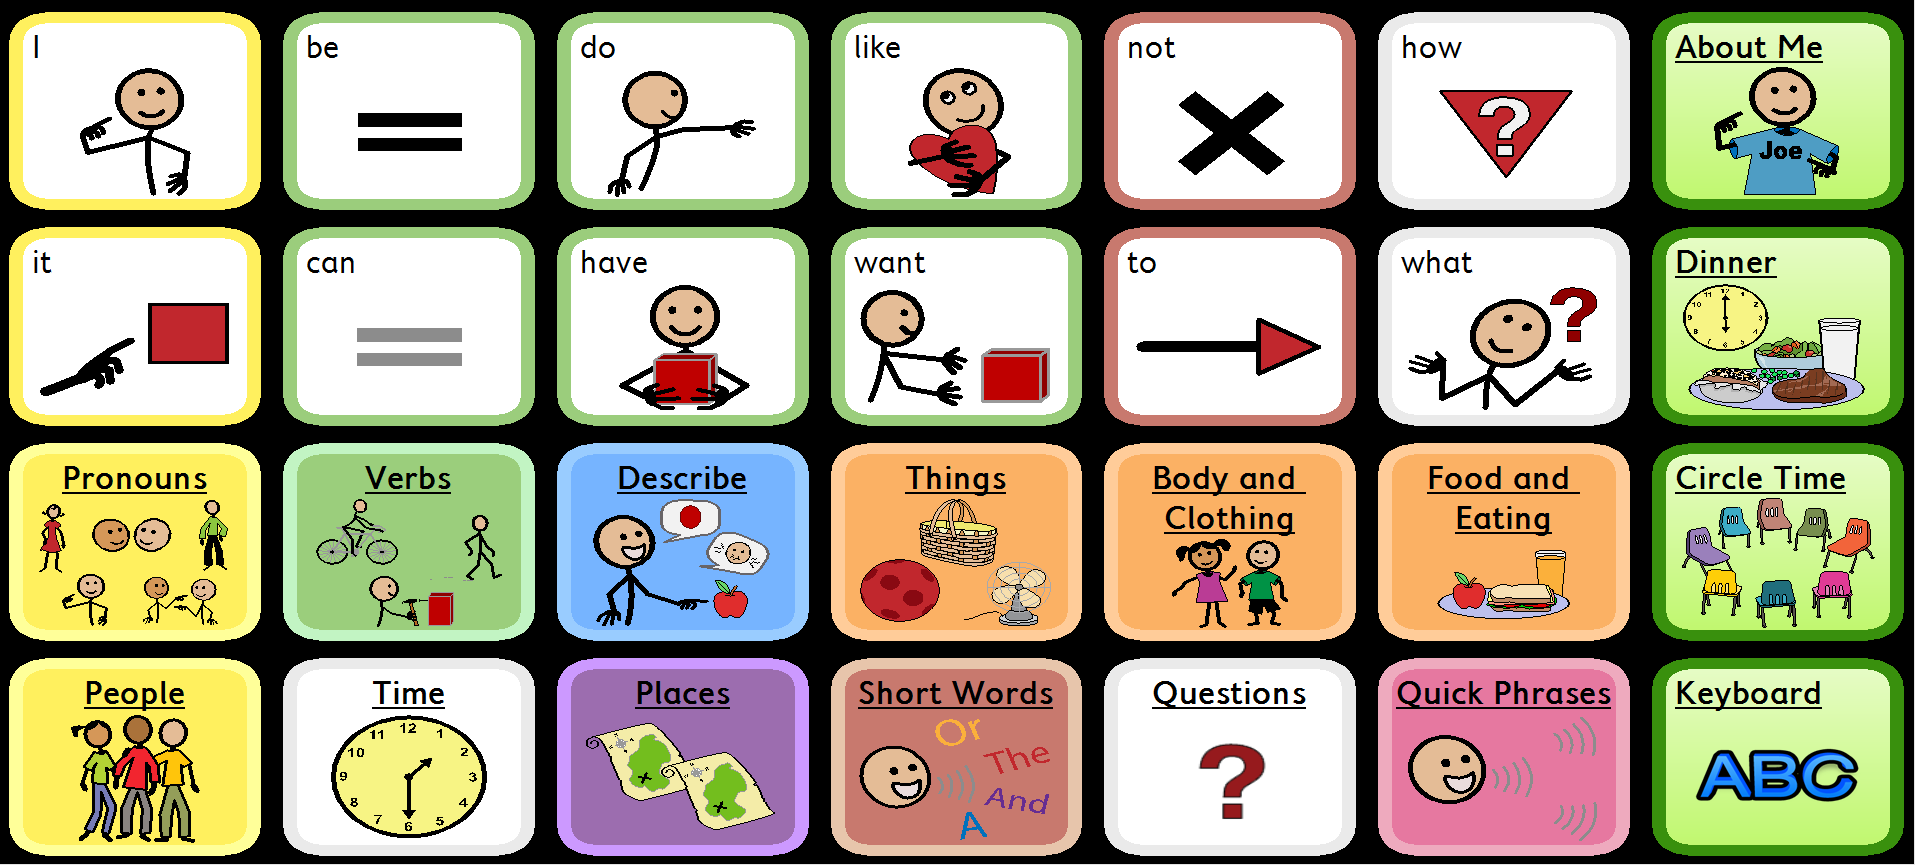
\includegraphics[width=100mm]{symbolgrid}
\caption{Skjermdump av symboltabellen til programvaren Sono Flex}
\label{fig:symbolgrid}
\end{figure}


\subsection{Brukerinteraksjon}

Sono Flex tilbyr to måter for brukerinteraksjon,  mus og øyestyring. Mus fungerer som vanlig ved at brukeren svever med musepekeren over ønsket knapp og venstreklikker for å aktivere. Ved øyestyring må brukeren fokusere blikket på ønsket knapp en gitt tid for at applikasjonen skal tolke det som et klikk. 

Det som skjer er at med engang brukeren fokuserer blikket på en knapp så starter en nedtelling. Figur \ref{fig:knapp-interaksjon} viser hvordan brukeren presenteres for hvor mye av nedtellingen som gjenstår.  Hvis brukeren ikke flytter blikket før nedtellingen har nådd null tolkes dette som et klikk.
For å gi brukeren beskjed om et godkjent klikk så dannes det en rød firkant rundt knappen. 

\begin{figure}[ht!]
\centering
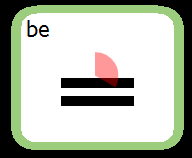
\includegraphics[width=50mm]{Knapp-interaksjon}
\caption{Skjermdump som viser hvordan nedtellingen på en knapp ser ut. Når den røde sirkelen er komplett oppfattes det som et klikk}
\label{fig:knapp-interaksjon}
\end{figure}


\section{Organisasjon og Navigasjon}

Som nevnt i seksjon \ref{subsec:navigasjon} så vil et barns vokabular være så stort at en nødvendigvis må fordele ordene over flere sider. Sono Flex har eksempelvis 106 ord under kategorien "Ting". Med tanke på at det maksimalt er plass til 28 ord på hver side så må disse fordeles og det må finnes en måte å navigere sidene. Løsningen har blitt en svært flat struktur med et hierarki på maksimalt 2 nivåer, ergo det finnes ikke underkategorier. Figur \ref{fig:hieraki-ting} viser hvordan dette fungerer i praksis. Når man trykker på kategorien "ting" så fylles tabellen med 27 ord som passer inn i kategorien "ting". Hvis man ikke finner ønsket ord på den første siden, navigerer man videre med knappen "neste side" og ordene i tabellen erstattes av nye ord. 


\begin{figure}[ht!]
\centering
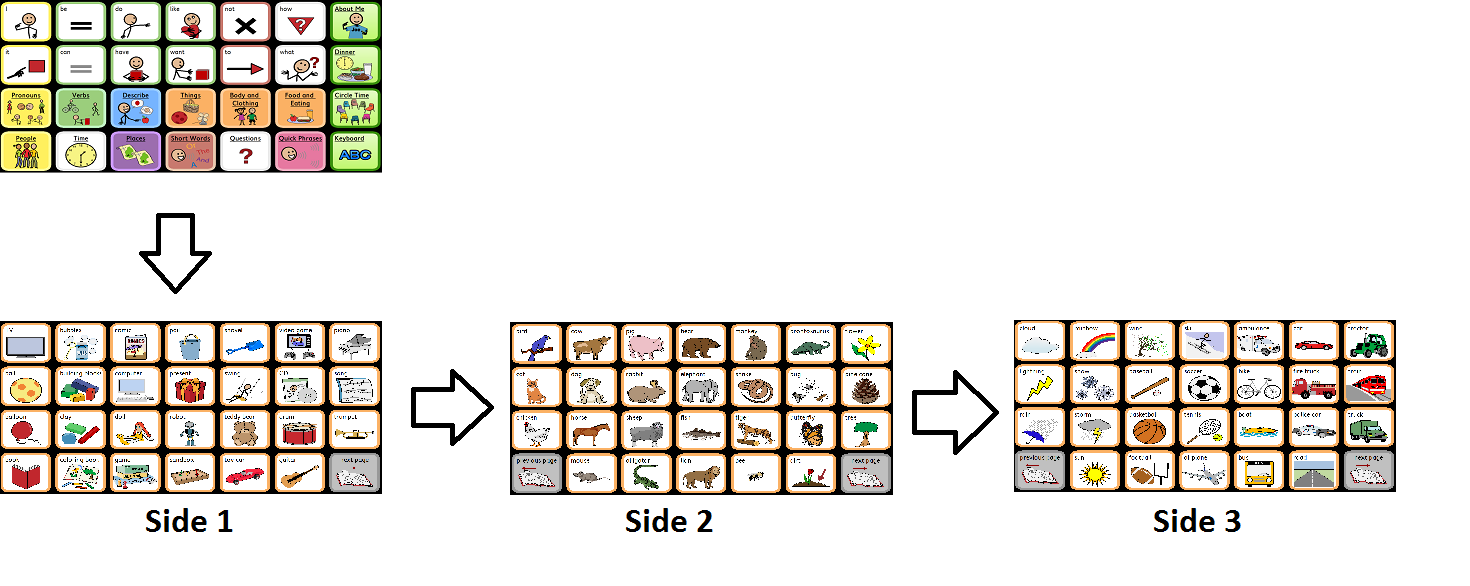
\includegraphics[width=140mm]{Symbgrid}
\caption{Skjermdump hierakiet til Sono Flex}
\label{fig:hieraki-ting}
\end{figure}







\chapter{Applikasjon}

I dette kapittelet vil det bli gjort rede for utviklingen og de applikasjonen.


\section{Utvikling}


Målet med forskningen er å undersøke potensielle forbedringer funksjonene beskrevet i seksjon \ref{sec:ResearchQuestion} kan ha på den eksisterende løsningen Tobii Sono Flex (\ref{chap:Tobii-Sono-Flex}). Det mest naturlige valget for å implementere disse funksjonene ville vært å ta utgangspunkt i den eksisterende kildekode og utvidet med nødvendig kode. Problemet var at plattformen som den eksisterende koden var bygget på hadde flere begrensninger og ville gjort det vanskelig å fått implementert mye av funksjonalitet som skulle undersøkes, spesielt gjelder det animasjonene. Dette gjorde at utviklingen ble startet som et nytt prosjekt og at første del av utviklingen var å lage en forenklet prototype av den samme applikasjonen bare på en annet rammeverk.

\subsection{Rammeverk}

Siden grunnen til at utviklingen begynte med blanke ark var begrensninger i det eksisterende rammeverket, var det viktig at den nye som applikasjonen skulle bygges på, ikke hadde dem. Valget ble derfor basert på at den var tilrettelagt for implementering av ønsket funksjonalitet. Det vil si god støtte for brukergrensesnitteknologi som animasjon, lyd og bildebruk. En annen viktig faktor var at rammeverket måtte være kompatibelt med øyestyringsenheten Tobii PCEye GO.
Valget falt derfor på Microsoft .NET. Grunnen til dette var at rammeverket oppfylte alle kravene og er godt dokumentert.


Arkitekturen til .NET er omfattende og som en kan se utifra figur \ref{fig:net-arkitektur} er det flere programmeringspråk og komponenter en kan velge å ta i bruk. Rapporten vil derimot kun gi informasjon om de ulike komponentene fra .NET som ble brukt og er nødvendig for videre lesning.


\begin{figure}[ht]
\centering
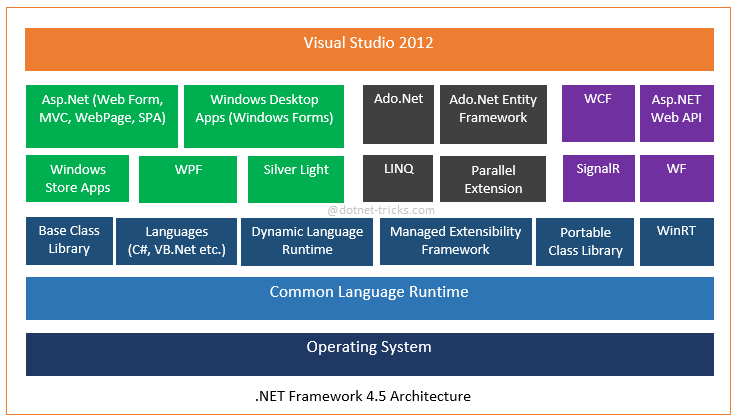
\includegraphics[width=140mm]{netframework45}
\caption{Diagram som viser arkitekturen til .net rammeverket versjon 4.5}
\label{fig:net-arkitektur}
\end{figure}

\subsection{Windows Presentation Foundation}

Det er hovedsaklig to delsett av .NET som er brukt til å utvikle applikasjonen, programmeringspråket C-sharp sammen med presentasjonssystemet Windows Presentation Foundation (\gls{WPF}).  WPF er et grafisk system for å lage brukergrensesnitt og tilhørende logikk til Windows-baserte applikasjoner som utnytter den grafiske maskinvaren best mulig. WPF bruker eXtensible Application Markup Language (\gls{XAML}), som er et XML-basert språk til å definere og kombinere ulike grensesnittelementer. Figur \ref{lst:myLabel} viser hvordan et vindu med en knapp er definert i XAML. Resultatet kan ses i figur \ref{fig:xamlButton}. 

\begin{lstlisting}[language=java,caption={Kodesnutt skrevet i XAML som viser en enkel applikasjon med en knapp}
\label{lst:myLabel}, belowcaptionskip=4pt]
<Window xmlns="http://schemas.microsoft.com/winfx/2006/xaml/presentation" Title="Window with Button"  Width="250" Height="100">

  <Button Name="button" Click="button_Click">Click Me!</Button>
  
</Window>
\end{lstlisting}

\begin{figure}[ht!]
\centering
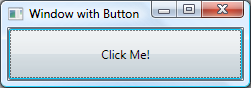
\includegraphics[width=100mm]{xamlButton}
\caption{Skjermdump av det applikasjonen som blir gjengitt ved kjøring av kodefnutt \ref{lst:myLabel}}
\label{fig:xamlButton}
\end{figure}


For å kunne samhandle med de grafiske objektene definert i XAML filen opprettes det alltid en tilhørende kodefil sammen med denne. Kodefilens formål er å ta seg av data og logikk for å ha et klart skille mellom utseende-spesifikk kode og oppførsel-spesifikk kode. For eksempel så vil en knapp sitt utseende og plassering bli definert XAML filen, mens hvordan data blir påvirket av interaksjon med knappen blir definert i den tilhørende kodefilen.



Den tilhørende kode-filen til XAML koden beskrevet i kodesnutt \ref{lst:myLabel} er vist i kodesnutt \ref{lst:backbutton}. Ved å trykke på knappen bildet vil metoden button\textunderscore Click i kodefilen bli kalt og en dialogboks vist til brukeren.

En XAML fil definerer som tidligere nevnt grafiske objekter som vindu, side eller brukerkontroll, men for at en bruker skal kunne samhandle med applikasjonen trengs de


Vindu inneholder er en konteiner som inneholder alle applikasjonens grafiske elementer. En

For å håndtere logikken og interaksjon med brukergrensesnittet,  definert i XAML, brukes det en kodefil. For hver XAML   Dette Dette gjør at koden har et klart skille mellom utseende-spesifikk kode og oppførsel-spesifikk kode.

Som tidligere nevnt defineres brukergrensesnittet i XAML,

WPF oppfordrer til å skille mellom utseende spesifikk kode og oppførsel-spesifikk kode ved at grafiske elementer skrives i XAML og interaksjonen  kun brukes til generere 
XAML brukes til å generere brukergrensesnitt, 
Hver XAML-fil har en tilhørende kode-fil for håndtering av hendelser og oppførsel. Dette gjør at koden har et klart skille mellom utseende-spesifikk kode og oppførsel-spesifikk kode. Den tilhørende kode-filen til XAML koden beskrevet i kodesnutt \ref{lst:myLabel} er vist i kodesnutt \ref{lst:backbutton}. Ved å trykke på knappen bildet vil metoden button\textunderscore Click i kodefilen bli kalt og en dialogboks vist til brukeren.

\begin{lstlisting}[language=java,caption={falafel}
\label{lst:backbutton}]
 void button_Click(object sender, RoutedEventArgs e)
        {
         Viser en dialogboks naar knappen trykkes
        MessageBox.Show("Hallo!");
        }
\end{lstlisting}





\section{Layout}

Beskriv den endelige layouten.
 - Mulighet for å endre antall rader og kolonner.

\section{Organisasjon}
Hvordan er applikasjonen organisert
Hvor mange lag det er  mulighet for


\section{}

Tobii Sono flex har 


I de neste seksjonene kommer jeg til å beskrive funskjoner som har blitt implementert.

\section{Animasjon}

Animasjoner i programvare brukes som et virkemiddel for å tiltrekke seg oppmerksomhet, underholde eller demonstrere noe. Det kan enten være en kort animasjon som at en knapp tilter til en side når man svever over den med musen eller det kan være av den lengre sorten som en elefant som står å danser. Animasjon er i hovedsak alt som beveger seg i applikasjonen. Selv om animasjoner kan fungere som et positivt virkemiddel gjør Nielsen og Loranger et poeng ut av at for mye blinkende og bevegende elementer kan slite ut brukeren og gjør det vanskeligere å fokusere på oppgaven. Det er nettopp dette animasjonene som er implementert skal finne ut av. Hvilke animasjoner fungerer som et hjelpemiddel og med det gir verdi til applikasjonen og hvilke som er distraherende for brukeren og gir en uønsket effekt.


Animasjonene i denne applikasjonen skjer som en respons til at brukeren trykker på et symbol. Hva som skjer avhenger av hvilken type symbol det er. De ulike typene som finnes i symboltabellen ble forklart i seksjon \ref{subsubsec:symboltabell} som ordsymbol, kategorisymbol og navigasjonssymbol. 


\subsection{Animasjoner: ordsymbol}
Når en bruker trykker på et ordsymbol, vil symbolet legge seg i setningslisten og er da klar for gjøres om til tydelig tale. I Sono Flex blir brukeren presentert for endringen ved at symbolet vises setningsfeltet. Prototypen ønsker å gi en mer visuell representasjon av denne endringen til brukeren. 

I) Symbolet flyter fra opprinnelig posisjon over de andre symbolene til setningsfeltet. 
II) Symbolet krympes,  i setningslisten vil det samme symbolet begynne som begynne som lite og vokse tilbake til samme størrelse. 

//vis bilder,  forklar animasjonene bedre. 

Med dette ønsker å blablabla

\subsection{Animasjon: Kategorisymbol}

\subsection{Animasjon: Navigasjonssymbol}


I prototypen ønsker animasjonen å vise hva som skjer,  ved at symbolet beveger seg fra opprinnelige posisjon til set

I Sono Flex dukker symbolet bare opp i setningslisten.

I symboltabellen er det 3 forskjellige typer. Man har 
ordsymbol, kategorisymbol og navigasjonssymbol. Et ordsymbol representerer selvsagt et ord og vil legge seg i listen sammen med andre ord som vil bli 

For å vise hva som skjer, fremfor at det bare skjer. I den eksisterende løsningen Sono Flex var det ingen for animasjoner. Slik at når brukeren trykte på en knapp, skjedde responsen umiddelbart. Man kan si at animasjonene skal representere det som skjer med dataen. Eksmepelvis hvis brukeren trykker på en knapp 


//tre ulike knapper
    //Trykk på knapp
    //neste side
    //Organisasjon



Det vil derfor være viktig at animasjonene som er implementert gir verdi til applikasjonen fremfor å distrahere.

Det vil derfor være viktig å finne ut om animasjonene gir noe verdi 

Interaksjonsdesigneren Nielsen har gjort flere undersøkelser på hvordan en skal få optimal brukervennlighet på webapplikasjoner. 

Animasjoner i programvare og nettsider blir ofte snakket om i negative ordlag fordi de

for det de ofte blir brukt overdrevet mye og er u

Animasjoner blir ofte sett på som en distraksjon når det blir brukt i applikasjoner for det de fjerner fokuset fra det som er viktig. Som 


For å kunne sjekke hvordan animasjon påvirket et barns evne til å samhandle med applikasjonen, måtte de ble implementert.  

//visualiserer at symbolet går fra griden til output, hjelper barnet
// Vanskeligheten med å skaffe empirisk data


Dataanimasjon, animasjonsfilmteknikk som gjør bruk av elektronisk databehandling for å skape illusjon av bevegelse, har fått en svært sentral plass innenfor reklamefilm og fjernsyn. Her har utviklingen gått fra enkle todimensjonale tegninger til avansert 3-D-animasjon som ikke kan fremstilles på andre måter enn med datamaskin.

Ifølge Store norsk leksikon defineres animasjon som levendegjørelse, besjeling, oppmuntring, tilskyndelse. 


Applikasjonen tilbyr flere animasjoner som brukeren kan velge mellom, enten alene eller flere i kombinasjon. Noen animasjoner kan ikke være operative samtidig ettersom det vil føre til konflikt. 

\subsection{Fade in, fade out}

Gjør rede for og forklar de ulike animasjonen

\section{Navigasjon}
Gjør rede for og forklar de forkjellige navigasjons hjelpemidlene

\section{Personlig tilpasning}
Forklar hvordan applikasjonen legger til rette for brukeren.
    - Temaer, forkjellige farger, lyder, 
    - Bruker kan velge hvilke animasjoner som ønskes og hurtigheten på dem.
    
\section{Lyd}
    Gjør rede for de ulike lydene.










\chapter{Dette er bare utkast og stikkord}

Rapporten vil ikke gi noen videre beskrivelse av C-Sharp, derimot vil WPF bli forklart.


\section{Teknologier}

Øyesporingsenheten beskrevet i kapittel  krever at systemet kjører på operativ systemet Windows og APIet som det leveres enheten leveres med,  fungerer kun i programmeringspråkene C-Sharp og C++. Med dette som utgangspunkt ble resten av teknologivalgene er basert på anbefalinger fra dokumentasjonen og tidligere erfaring. 


\begin{description}
  \item[IDE] Visual Studio
  \item[Rammeverk] .NET
  \begin{description}
     \item[Programmeringspråk] C\#
     \item[Grafikk] Windows Presentation Foundation 
\end{description}
  \item[Versjonskontroll] Git (BitBucket)
\end{description}


Fitzergald key, personliggjør keyboardet med farger. Viktigste er at det er konsistent


For å kunne bruke symboler som en kommunikasjonsform kreves det at brukeren har mulighet til samhandle med dem. For å få til dette brukes det en øyestyringsenhet koblet til en datamaskin som fanger opp brukerens pupill bevegelser. På den måten erstatter øyene den vanlige musepekeren.

\subsubsection{Kalibrering}


Første gang en kobler øyestyringsenheten til maskinen, anbefales det at brukeren gjør en oppmåling og kalibrering for mer presis øyesporing. Oppmålingen innebærer at personen måler størrelsen på skjermen - kalibreringen at det brukeren bes om å følge en prikk som traveserer skjermen. Ettersom dette vil gi øyestyringsenheten et referansepunkt. Prosessen er kun nødvendig første gang for gjeldene bruker. 






Dette gir tilgang på deres application programming interface (API), herved referert til som Tec API. Tec API gjør funksjoner og informasjon fra sporingsenheten tilgjengelig. 


The Tobii Eye Control API provides two alternative access points: a .NET assembly and a C dynamic-link library. Both alternatives
give the developers of eye controlled applications access to the functionality of the Gaze Interaction Server. The .NET API also
contains specialized interaction support for common user interface frameworks such asWindows Presentation Foundation
(WPF) andWindows Forms. The C interface, called MPACI, provides backward compatibility with older Tobii products such as
the MyTobii software.




\subsection{Systemkrav}

\subsection{Nøkkelfunksjoner og konsepter}

\section{}

Første gang en kobler til må en gå igjennom ett oppsett. Dette innebærer måling av den aktuelle skjermen som brukes og en kalibrerings rutine. For å oppnå nøyaktig øyesporing.  

For en førstegangsbruker av enheten anbefales det å gjøre en kalibrering, for optimal opplevelse. Informasjonen


Øyestyringsenheten som er illustrert i figur \ref{fig:tobiiPc}  . Denne




\medskip

\bibliographystyle{chicago}%Used BibTeX style is unsrt
\bibliography{sample}

\end{document}
